% Figure used: task2_benchmark.png
\section{Task 2: Adversarial Search in Tank Battle}

\subsection{Zero-Sum Game Formulation}
The turn-based Tank Battle game is formulated as a deterministic, two-player, perfect-information zero-sum game in which Player~1 acts as \textbf{MAX} (maximizing utility) and Player~2 acts as \textbf{MIN} (minimizing MAX's utility). The formal components are defined as follows:

\begin{itemize}
    \item \textbf{Game State ($s \in S$):} At each game cycle, a state is represented by $s = \langle T_1, T_2, B_1, B_2, \mathcal{W}, \mathcal{M}, \text{turn} \rangle$, where $T_i = (x_i, y_i, d_i, hp^T_i)$ denotes the position, facing direction $d_i \in \{\text{UP, DOWN, LEFT, RIGHT}\}$, and health of Tank~$i$ (initial $hp^T = 6$); $B_i = (x^B_i, y^B_i, hp^B_i)$ denotes the position and health of Base~$i$ (initial $hp^B = 9$); $\mathcal{W} = \{(x_w, y_w, hp_w)\}$ is the set of destructible brick walls (initial $hp_w = 3$); $\mathcal{M}$ is the list of active bullets; and $\text{turn} \in \{1, 2\}$ specifies the active player.
    \item \textbf{Actions ($A(s)$):} On each turn, the active tank can select from up to six legal actions: $\text{MOVE\_UP}$, $\text{MOVE\_DOWN}$, $\text{MOVE\_LEFT}$, $\text{MOVE\_RIGHT}$, $\text{FIRE}$, and $\text{STAY}$. A movement action updates the tank's orientation and advances it by one cell if the target cell is not blocked by map boundaries, walls, bases, or the opponent's tank; if blocked in a different direction, the tank is still permitted to rotate in place.
    \item \textbf{Transition Function ($\text{Result}(s, a)$):} Executing action $a$ in state $s$ first applies the active tank's movement (including immediate collision resolution if the tank steps onto an active bullet) or spawns a new bullet on $\text{FIRE}$. Next, all active bullets advance up to three cells per game cycle, checked cell by cell; upon hitting a wall, tank, or base, the target loses $1\text{ HP}$ and the bullet is removed immediately.
    \item \textbf{Terminal Test and Utility Function ($U(s)$):} A state is terminal when either tank or either base is destroyed ($hp \le 0$), or when the turn limit $T_{\max} = 200$ is reached. The utility for MAX is:
    \begin{equation}
    U(s) = \begin{cases}
    +10000 & \text{if only MIN is defeated } (hp^T_2 \le 0 \lor hp^B_2 \le 0), \\
    -10000 & \text{if only MAX is defeated } (hp^T_1 \le 0 \lor hp^B_1 \le 0), \\
    0 & \text{if both are defeated or } T_{\max} \text{ is reached.}
    \end{cases}
    \end{equation}
\end{itemize}

\subsection{Adversarial Search Algorithms and Heuristic Evaluation}
Because full matches span dozens of turns and the branching factor reaches up to $6$, Pure Minimax (MM) and Pure Alpha-Beta Pruning (AB) cannot reach terminal states within real-time depth bounds during mid-game play. We therefore apply depth-limited search (cutoff depth $d$) paired with a five-component tactical evaluation function:
\begin{equation}
\text{Eval}(s) = S_{\text{hp}} + S_{\text{pos}} + S_{\text{shield}} + S_{\text{aim}} + S_{\text{bullet}}.
\end{equation}
From the perspective of the evaluating agent ($\text{my}$) against its opponent ($\text{opp}$):
\begin{itemize}
    \item \textbf{Health Advantage ($S_{\text{hp}}$):} $S_{\text{hp}} = 170\,hp^T_{\text{my}} - 210\,hp^T_{\text{opp}} + 200\,(hp^B_{\text{my}} - hp^B_{\text{opp}})$, prioritizing offensive pressure and base defense, with an additional survival penalty $-120\,(3 - hp^T_{\text{my}})$ when $hp^T_{\text{my}} \le 2$.
    \item \textbf{Wall-Aware Distance ($S_{\text{pos}}$):} Instead of raw Manhattan distance, we compute weighted shortest-path distances $d_W$ via Dijkstra's algorithm (empty cell cost $1$; wall cell cost $hp_w + 1$, reflecting shots to breach plus movement; non-target base cells impassable), cached once per wall configuration for $O(1)$ lookup during tree search:
    \begin{equation*}
    S_{\text{pos}} = -w_c\,d_W(T_{\text{my}}, T_{\text{opp}}) - 8\,d_W(T_{\text{my}}, B_{\text{opp}}) + 5\,d_W(T_{\text{opp}}, B_{\text{my}}),
    \end{equation*}
    with $w_c = 14$ when $hp^T_{\text{opp}} \le 2$ to encourage decisive finishing and $w_c = 6$ otherwise.
    \item \textbf{Base Shield Integrity ($S_{\text{shield}}$):} $S_{\text{shield}} = 12\,(W_{\text{my}} - W_{\text{opp}})$, where $W_i$ is the total HP of walls orthogonally adjacent to Base~$i$.
    \item \textbf{Line of Sight ($S_{\text{aim}}$):} Rewards clear line-of-sight alignment toward the enemy tank or base ($+45/+50$ within immediate 3-cell bullet range, $+25/+30$ beyond) and penalizes exposure to enemy aim ($-40/-45$ within 3 cells, $-20/-25$ beyond).
    \item \textbf{Active Bullets ($S_{\text{bullet}}$):} Applies heavy penalties ($-90/-70$) when an enemy bullet has a clear trajectory toward our tank or base to induce dodging, and rewards ($+70/+60$) well-aimed friendly bullets.
\end{itemize}

Two search optimizations are incorporated into the heuristic and Alpha-Beta variants: (i)~depth-adjusted terminal scores ($\pm 10 \cdot \text{depth}$) to prefer faster wins and delay losses, and (ii)~context-aware \textbf{Move Ordering}, which prioritizes $\text{FIRE}$ only when an enemy target or wall lies ahead of the barrel (preventing wasted shots on ties), combined with 1-ply heuristic sorting at the root for Heuristic Alpha-Beta to trigger early cutoffs ($\beta \le \alpha$).

\subsection{Experiments and Discussion}
All four configurations---Minimax (MM), Alpha-Beta (AB), Heuristic Minimax (H-MM), and Heuristic Alpha-Beta (H-AB)---were implemented following Object-Oriented Programming principles. Each timing measurement is averaged over $5$ repeated runs after $1$ warm-up run. The agents were benchmarked on two symmetric scenarios, \textit{Endgame ($2\text{ HP}$ Tank, $2\text{ HP}$ Base)} and \textit{Mid-game ($6\text{ HP}$ Tank, $9\text{ HP}$ Base)}, across depths $d \in \{2, 3, 4, 5\}$, followed by a full-match tournament including side-swapped matchups on the Mid-game ($9\times 9$) and Battle City ($13\times 13$) maps.

\begin{table}[htbp]
\caption{Search Performance Comparison on the Mid-game Scenario ($6\text{ HP}$).}
\begin{center}
\begin{tabular}{|l|c|r|r|c|}
\hline
\textbf{Algorithm} & \textbf{$d$} & \textbf{Nodes} & \textbf{Time (ms)} & \textbf{Action} \\
\hline
Minimax & 2 & 42 & 0.615 & FIRE \\
Alpha-Beta & 2 & 17 & 0.141 & FIRE \\
Heuristic MM & 2 & 42 & 3.345 & MOVE\_DOWN \\
Heuristic AB & 2 & 17 & 1.769 & MOVE\_DOWN \\
\hline
Minimax & 3 & 252 & 1.316 & FIRE \\
Alpha-Beta & 3 & 57 & 0.465 & FIRE \\
Heuristic MM & 3 & 252 & 8.448 & MOVE\_DOWN \\
Heuristic AB & 3 & 70 & 4.555 & MOVE\_DOWN \\
\hline
Minimax & 4 & 1{,}477 & 9.091 & FIRE \\
Alpha-Beta & 4 & 126 & 1.268 & FIRE \\
Heuristic MM & 4 & 1{,}477 & 38.176 & MOVE\_DOWN \\
Heuristic AB & 4 & 181 & 10.977 & MOVE\_DOWN \\
\hline
Minimax & 5 & 8{,}512 & 48.598 & FIRE \\
Alpha-Beta & 5 & 361 & 4.038 & FIRE \\
Heuristic MM & 5 & 8{,}512 & 184.310 & MOVE\_DOWN \\
Heuristic AB & 5 & 634 & 29.769 & MOVE\_DOWN \\
\hline
\end{tabular}
\label{tab:task2_perf}
\end{center}
\end{table}

\begin{table}[htbp]
\caption{Full-Match Tournament Results (Including Side-Swapped Matchups).}
\begin{center}
\begin{tabular}{|l|c|c|c|c|}
\hline
\textbf{Matchup (P1 vs.\ P2)} & \textbf{Winner} & \textbf{Turns} & \textbf{HP (P1 / P2)} & \textbf{Avg.\ Nodes} \\
\hline
H-AB ($d{=}4$) vs.\ Pure AB ($d{=}4$)$^a$ & P1 & 37 & 6/9 vs.\ 6/0 & 137 / 115 \\
Pure AB ($d{=}4$) vs.\ H-AB ($d{=}4$)$^a$ & P2 & 38 & 6/0 vs.\ 6/9 & 115 / 159 \\
H-AB ($d{=}4$) vs.\ H-MM ($d{=}3$)$^b$ & P1 & 45 & 6/9 vs.\ 6/0 & 137 / 232 \\
H-MM ($d{=}3$) vs.\ H-AB ($d{=}4$)$^b$ & P2 & 46 & 6/0 vs.\ 6/9 & 237 / 163 \\
H-AB ($d{=}4$) vs.\ Pure MM ($d{=}3$)$^b$ & P1 & 55 & 6/9 vs.\ 1/0 & 140 / 242 \\
\hline
\multicolumn{5}{l}{\footnotesize $^a$Mid-game map ($9\times 9$). \quad $^b$Battle City map ($13\times 13$).}
\end{tabular}
\label{tab:task2_tour}
\end{center}
\end{table}

\begin{figure}[htbp]
\centerline{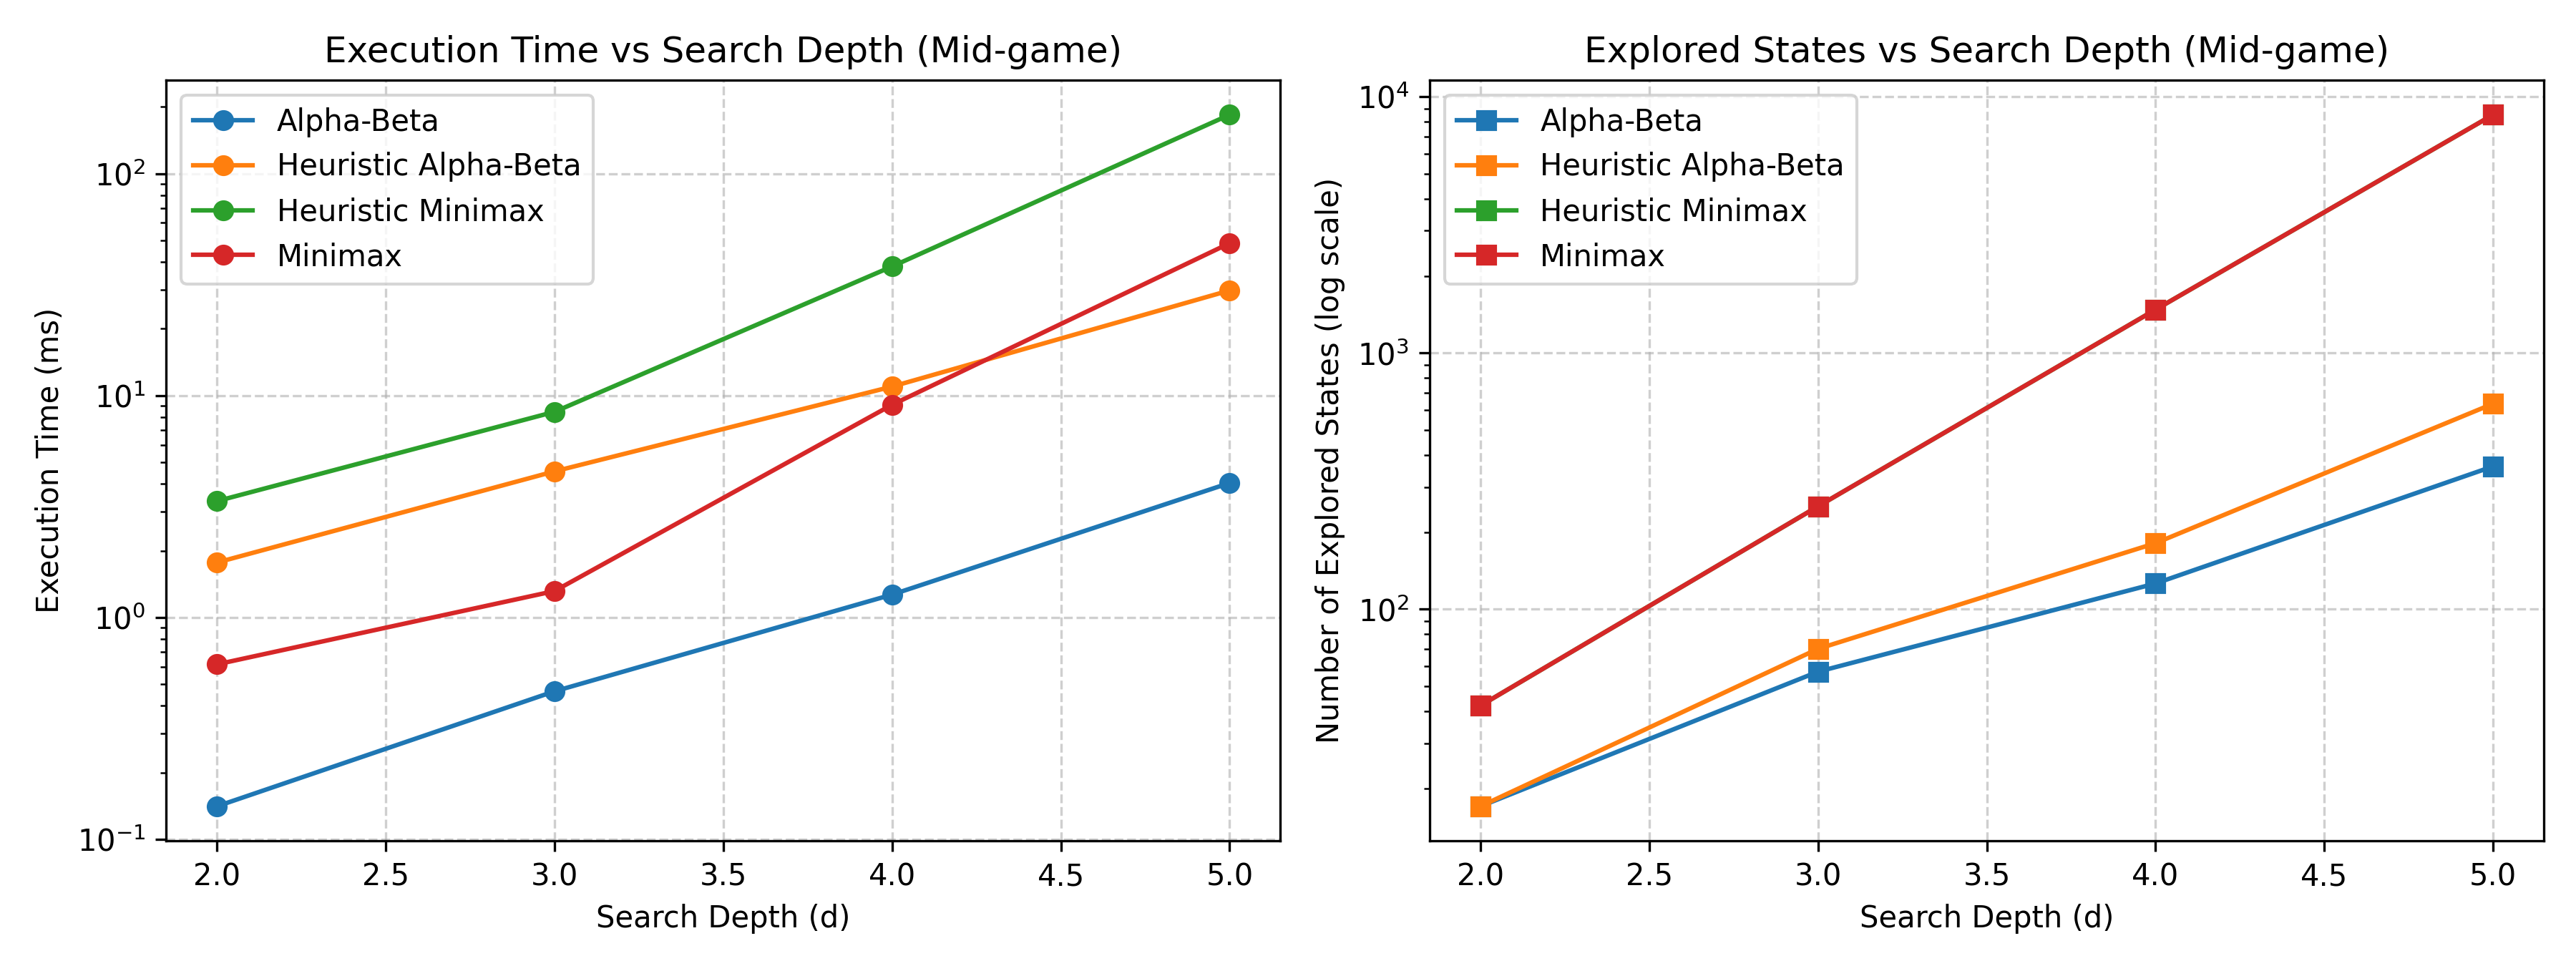
\includegraphics[width=\columnwidth]{task2_benchmark.png}}
\caption{Execution time and number of explored states versus search depth on the Mid-game scenario (log scale).}
\label{fig:task2_bench}
\end{figure}

From Table~\ref{tab:task2_perf}, Table~\ref{tab:task2_tour}, and Fig.~\ref{fig:task2_bench}, four main conclusions follow:
\begin{enumerate}
    \item \textbf{Effectiveness of Alpha-Beta Pruning with Move Ordering:} On the Mid-game scenario, H-AB reduces explored states compared to H-MM by $87.7\%$ at $d = 4$ ($181$ vs.\ $1{,}477$ nodes) and by $92.6\%$ at $d = 5$ ($634$ vs.\ $8{,}512$ nodes), cutting execution time at $d = 5$ by $6.2\times$ ($29.77\text{ ms}$ vs.\ $184.31\text{ ms}$) to enable smooth real-time PyGame play.
    \item \textbf{Impact of Heuristic Evaluation:} On the Mid-game scenario, Pure MM and Pure AB cannot reach terminal states within $d \le 5$, receiving $0$ at every leaf. Because all branches tie at $0$, Pure AB triggers trivial $\beta \le \alpha$ ($0 \le 0$) cutoffs immediately and explores fewer nodes than H-AB ($361$ vs.\ $634$ at $d = 5$), yet plays blindly and defaults to unproductive $\text{FIRE}$ actions, whereas H-MM and H-AB immediately select the tactical advance $\text{MOVE\_DOWN}$. On the decisive Endgame scenario ($2\text{ HP}$ Tank, $2\text{ HP}$ Base), only H-MM and H-AB identify the winning move $\text{MOVE\_DOWN}$ at $d \le 4$, while at $d = 5$ all four algorithms detect the forced base-destruction terminal state; at $d = 5$, H-AB explores $344$ vs.\ $7{,}794$ nodes for H-MM ($95.6\%$ reduction; $6.92\text{ ms}$ vs.\ $126.11\text{ ms}$, or $18.2\times$ faster) and even prunes more effectively than Pure AB ($344$ vs.\ $420$ nodes) thanks to heuristic move ordering.
    \item \textbf{Search-Depth Advantage Independent of First-Mover Bias (Table~\ref{tab:task2_tour}):} H-AB ($d = 4$) wins all five tournament matchups, including both side-swapped pairs. On the tactical Battle City ($13\times 13$) map, H-AB ($d = 4$) defeats H-MM ($d = 3$) cleanly ($6/9$ vs.\ $6/0$) both as Player~1 (45 turns; 137 vs.\ 232 nodes/turn) and as Player~2 (46 turns; 163 vs.\ 237 nodes/turn), proving that the victory stems from deeper lookahead enabled by Alpha-Beta pruning rather than first-mover advantage.
    \item \textbf{GUI and External Agent Integration:} The PyGame interface supports all four built-in algorithms, three selectable maps (Endgame, Mid-game, Battle City), and dynamic loading of external Python agents (\texttt{ExternalAgent}) for head-to-head evaluation in the same environment.
\end{enumerate}